
\documentclass[12pt]{article}
\pagestyle{empty}
\setlength{\parskip}{0in}
\setlength{\textwidth}{6.8in}
\setlength{\topmargin}{-.5in}
\setlength{\textheight}{9.3in}
\setlength{\parindent}{0in}
\setlength{\oddsidemargin}{-.7cm}
\setlength{\evensidemargin}{-.7cm}

\usepackage{amsmath}
\usepackage{amsthm}
\usepackage{amstext}

\usepackage{graphicx}

\begin{document}


\textbf{MAT 105 Exam 1 (ivory) Summer 2012} \hspace{.4in} {\large Name} \hrulefill

\begin{center}

\begin{tabular}
{|l|c|c|c|c|c|c|c|c|c|c|c|c|c|} \hline

 Problems & \hspace{5 pt} 1 \hspace{5 pt}  & \hspace{5 pt} 2 \hspace{5 pt} & \hspace{5 pt} 3 \hspace{5 pt} & \hspace{5 pt} 4 \hspace{5 pt} & \hspace{5 pt} 5 \hspace{5 pt} & \hspace{5 pt} Total  \hspace{5 pt} & &  \hspace{5 pt} Grade \hspace{5 pt}  \\ \hline
&&&&&&&&\\  
Points &&&&&&&    \hspace{.8in}\% &  \\ 
&&&&&&&& \\  \hline
Out of & 12 & 32 & 32 & 14 & 10 &100 & & \\ \hline

\end {tabular}

\end{center}

\vspace{.2in}

 \emph{Relax.  You have done problems like these before.  Even if these problems look a bit different, just do what you can.  If you're not sure of something, please ask! You may use your calculator.  Please show all of your work and write down as many steps as you can.  Don't spend too much time on any one problem.  Always remember to report the units on an answer. Do well.  And remember, ask me if you're not sure about something.} \\

\vspace{.5in} 
\noindent \emph{A few formulas from our book:}
\begin{center}

\textbf{Root Formula:} 

A solution of the equation $B^n=k$ is $B=k^{1/n}$.

\vspace{.2in} 

\textbf{Percent Increase Formula:} 

To get the result of increasing an amount by $r$\%, multiply by $1 + \frac{r}{100}$.

\end{center}

\hrulefill

%%%%%%%%%%%

\newpage

\begin{enumerate}

%%% Old 1.3, pop culture, fun
\item The song ``Someone Like You'' by Adele was a top song of 2011.  The graph below shows its ranking on the ARC Weekly Top 40 Countdown.  The song entered the countdown on August 20, 2011.


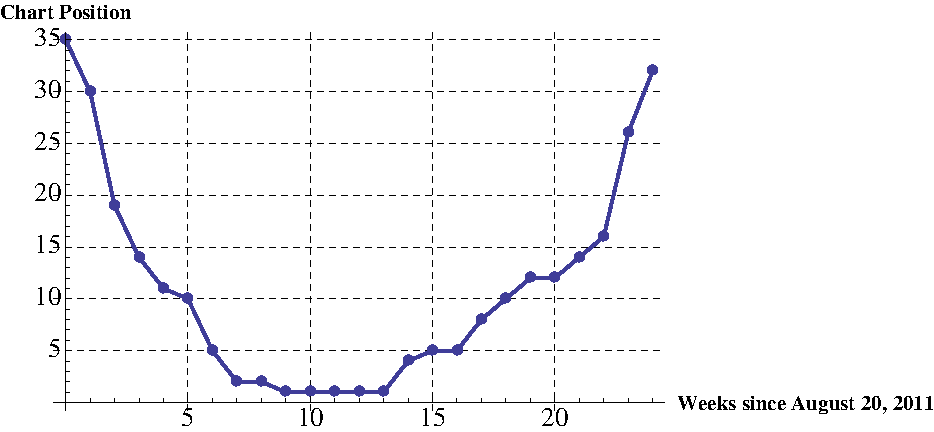
\includegraphics [width = 6in] {adele}

\begin{enumerate}
\item Does this graph show a dependency that is increasing, decreasing, or neither?
\vfill
\item After 16 weeks on the chart, what was the approximate ranking of the song?
\vfill
\item How many weeks did it take for the song to enter the top 10?  When did it leave the top 10?
\vfill
\item The last three weeks on the chart, the song's position changed 16 positions.  What do you think caused such a rapid drop in the rankings?  Please write a sentence explaining your answer.
\vfill
\end{enumerate}




\newpage
%%%%%%%%%%%%%%%%%%%%%%%%%
%%% Old 1.6, home, everyday
\item  To ship a package to my sister in Denver there is a flat rate of \$3.00 with a cost of \$0.15 for every ounce.  

\begin{enumerate}
\item Make a table showing the cost to ship the package if it weighs 5 ounces, 10 ounces, and 20 ounces. 
\vfill
\item Name the variables, including units, and write an equation illustrating the dependence.
\vfill
\item The postal worker told me it would cost \$5.70 to ship the package.  Solve your equation to determine how much the package weighs.  \emph{If you cannot solve the equation, you may show some other method of finding the answer for possible partial credit.}
\vfill
\item Draw a graph showing how the cost of the package changes with its weight. Be sure to (a) label your axes, (b) scale your axes appropriately to fill the entire graph paper, and (c) include all of the data in your table.
\vspace{.1in}
\begin{center}
\scalebox {.8} {
\includegraphics [width = 6in] {../graphPaper}}
\end{center}
\vspace{.1in}
\end{enumerate}
%%%%%%%%%%%%%%%%%%%%%%%%%%%%%%%%%%%
\newpage

%%% Old 1.8, wedding, everyday
\item The price of a wedding is increasing by 3\% per year.  In 2012, the average cost for a wedding in 2012 is approximately \$26,000 (= 26 thousand dollars).    
%
\begin{enumerate}
\item Write an equation illustrating this dependence using the following variables:

\quad $C= $ cost of a wedding (measured in thousands of dollars)

\quad $Y = $ year (measured in years since 2012)

\vfill
\item Make a table showing the cost of a wedding when $Y=0$ (the year 2012),  $Y=5$ (the year 2017),  $Y=10$ (the year 2022),  $Y=15$ (the year 2027). Please report your answer to the nearest whole thousand dollars.
\vfill
%\item Draw a graph showing how the cost of a wedding will change in the future.
%\vspace{.1in}
%\begin{center}
%\scalebox {.8} {
\includegraphics [width = 6in] {../GraphPaper}}
%\end{center}
%\vspace{.1in}
\item Use successive approximations to predict when the cost of a wedding will rise above 37 thousand dollars.   \emph{Display your work in a table.  Answer to the nearest year.  Be sure to say the actual year.}
\vfill

\end{enumerate}


%%%%%%%%%%%%%%%%%
\newpage
%%% Old 1.7, physics, everyday
\item When you apply the brakes to stop a bicycle, you don't actually stop immediately.  The distance it takes depends on how fast you were going.  For one bike tested, $D = 0.23 * S^2$, where $S$ is the speed of the bike (in mph) and $D$ is the distance before stopping (in feet).

\begin{enumerate}
\item Make a table showing the shopping distances for speeds of 5, 10, 15, and 20 mph.  Please report your answer to the first decimal place.
\vfill
\item Approximately how fast can a bike go and still be able to stop within 30 feet?  Please report your answer to the first decimal place.

\emph{You may use whatever method you prefer to answer the question, but please give an answer accurate to one decimal place.}
\vfill

\end{enumerate}



\noindent \hrulefill
%%% Old 1.4, gas prices, fun
%% http://en.wikipedia.org/wiki/Gasoline_and_diesel_usage_and_pricing
\item In South Korea, gasoline prices are recorded in wons/liter.  (The won is the currency of South Korea).  The average price of gasoline in South Korea is 2043 wons/liter.  What would that price be in terms of US dollars per gallon? (\emph{In other words, convert 2043 wons per liter to dollars per gallon.  I have started the unit conversion for you below.})


\emph{Useful facts:  \$1.00 $\approx$ 1171 wons and 1 gallon $\approx$ 3.8 liters }\vfill


\vspace{0.1in}

$ \displaystyle \frac{ 2043 \mbox{ wons } }{1 \mbox{ liter } }$
\vfill


\end{enumerate}



%%%%%%%%%%%%%%%%





\end{document}
